\documentclass{beamer}

\usepackage{graphics}

\title{Introduction to Machine Learning}
\author{Joseph P. Vantassel}
\institute{The University of Texas at Austin}
\date{2021}

\begin{document}

\frame{\titlepage}


\begin{frame}

\frametitle{Terminology}

What are the differences between Artificial Intelligence, Machine Learning, and Deep Learning?

\begin{center}
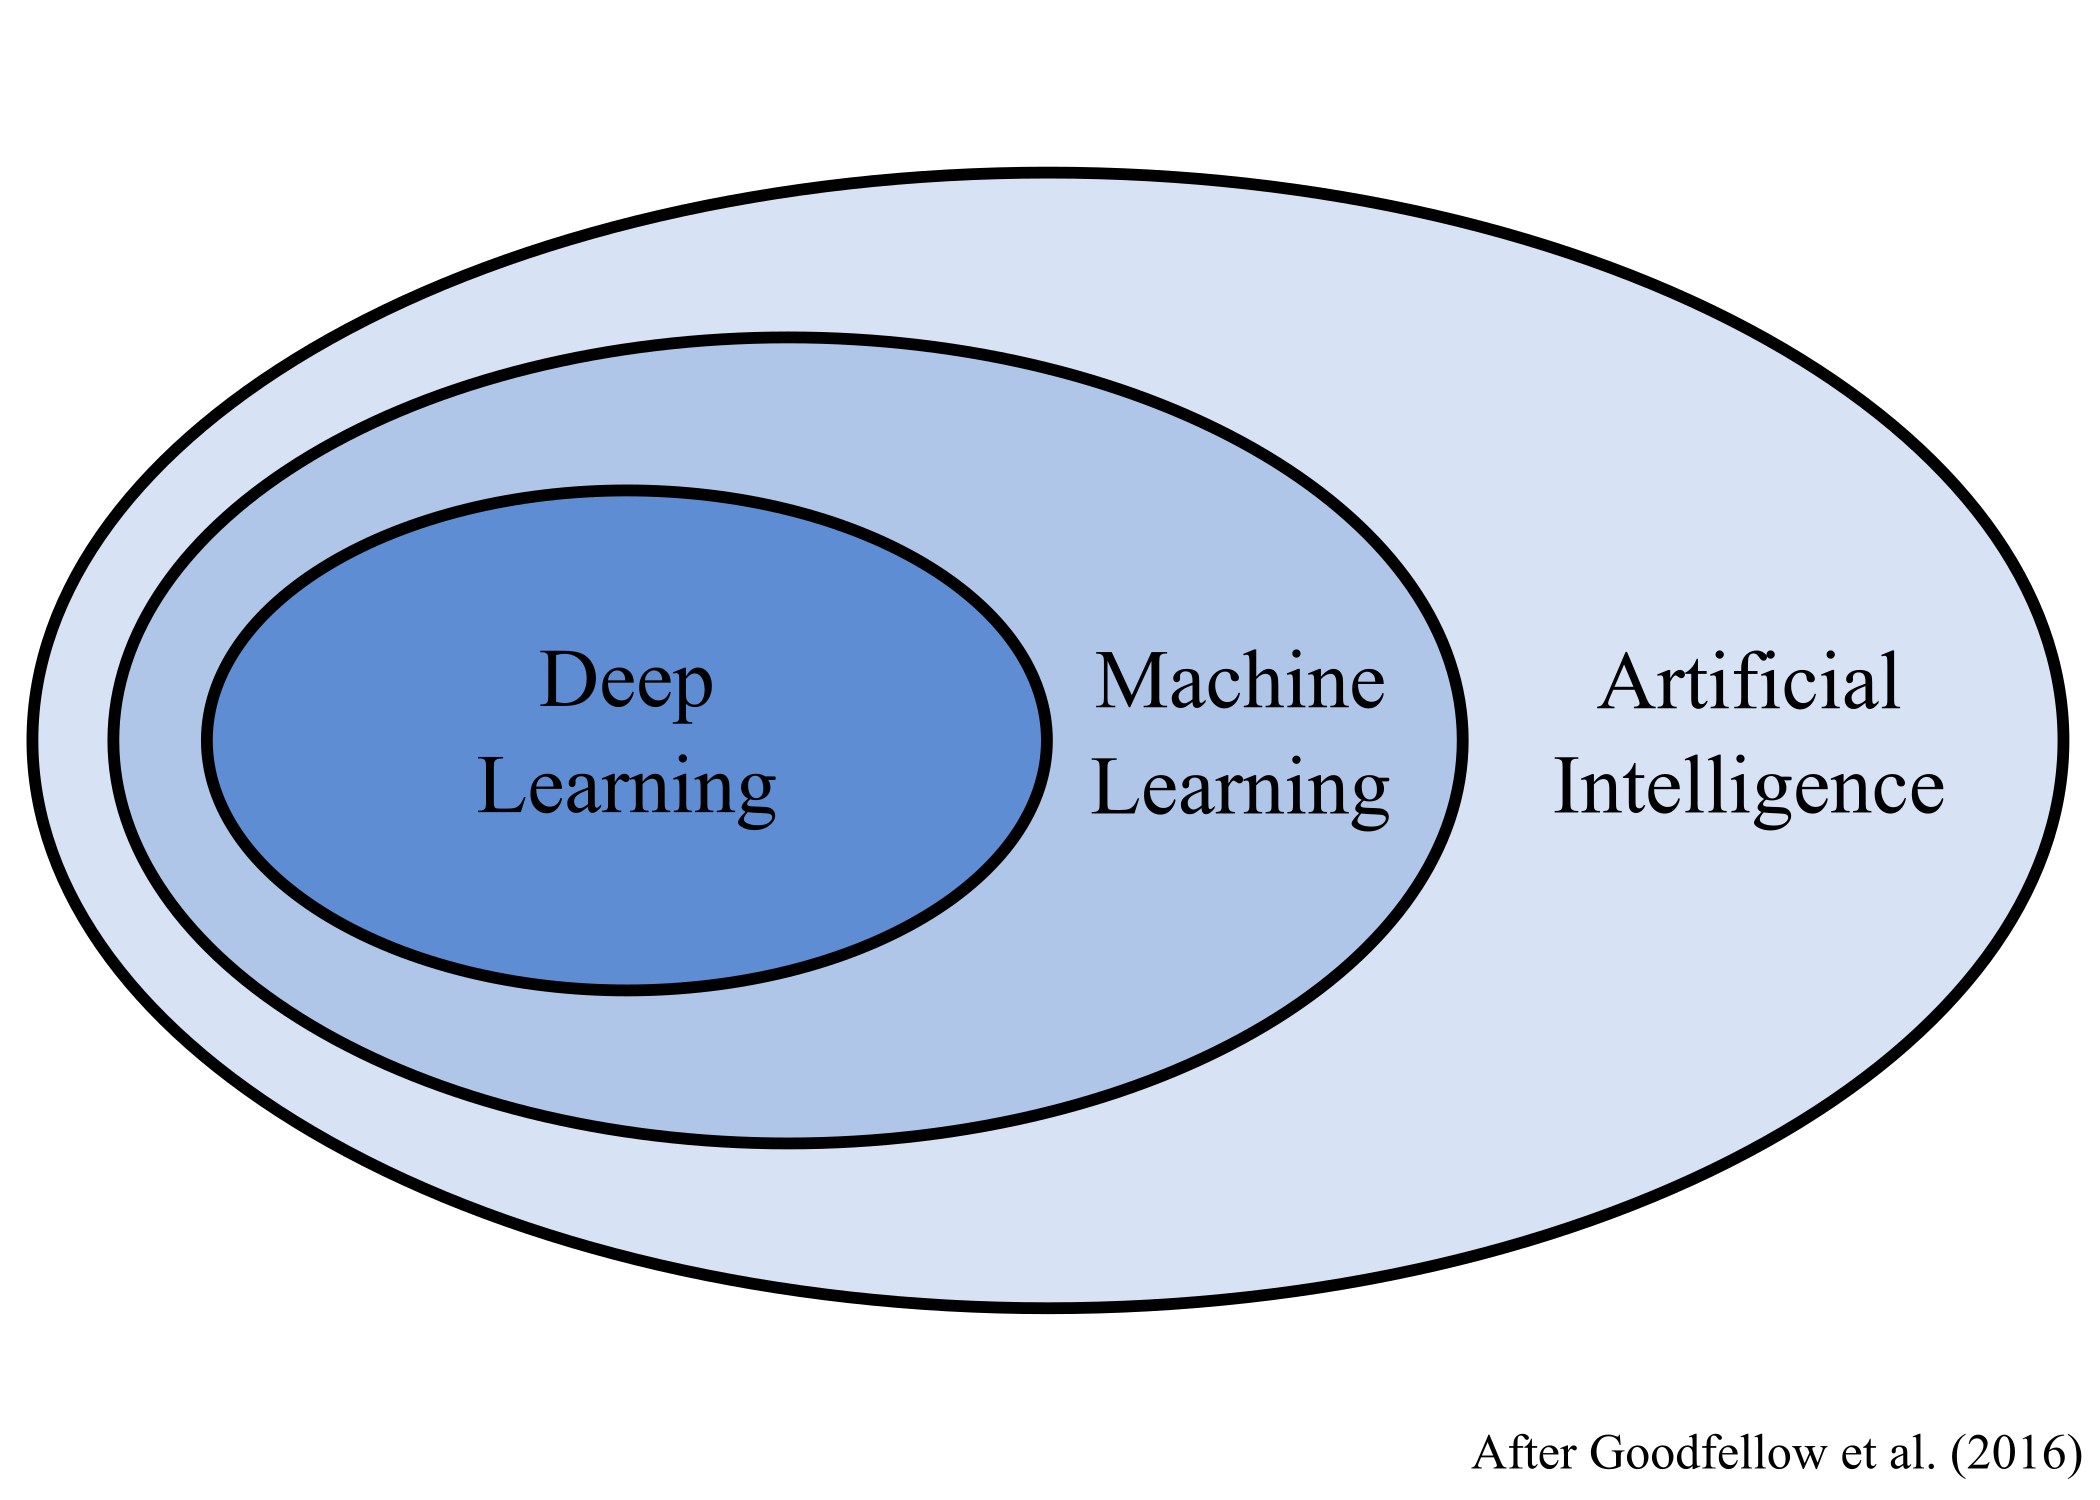
\includegraphics[height=5cm]{figs/ai_ml_dl_diagram.png}
\end{center}

\end{frame}


\begin{frame}

\frametitle{Artifical Intelligence (AI)}

\begin{itemize}
    \item Started in 1950's.
    \item Includes algorithms that allows computers to act intelligently.
    \item Early work focused on rule-based controllers.
\end{itemize}

\end{frame}


\begin{frame}

\frametitle{Machine Learning (ML)}

\begin{itemize}
    \item Started in 1980's.
    \item Includes algorithms that allows computers to teach themselves using simple pre-defined schemes.
    \item Examples:
    \begin{itemize}
        \item Support Vector Machines (SVM)
        \item K - Nearest Neighbor Classification
    \end{itemize}
\end{itemize}

\begin{block}{Definition - \textit{Mitchel T. (1997)}}
    Machine learning describes the process by which a computer adapts
    from experience \textbf{E}, on task \textbf{T}, to improve
    performance \textbf{P}.
\end{block}

\end{frame}


\begin{frame}

    \frametitle{Deep Learning (DL)}

    \begin{itemize}
        \item Started in 2010's.
        \item Special subclass of ML algorithm with potential for high-dimensional representations.
        \item Replaces simple pre-defined schemes with simple composable units.
        \item Examples:
        \begin{itemize}
            \item Multilayer Perceptrons (MLP)
            \item Convolutional Neural Networks (CNN)
            \item Long Short-Term Memory (LSTM)
        \end{itemize}
    \end{itemize}

\end{frame}

\begin{frame}

    \frametitle{Diggin In}

    \begin{block}{Definition - \textit{Mitchel T. (1997)}}
        ``Machine learning describes the process by which a computer adapts
        from experience \textbf{E}, on task \textbf{T}, to improve
        performance \textbf{P}.''
    \end{block}

    \vskip20pt

    \begin{itemize}
        \item Task, T
        \begin{itemize}
            \item the problem we hope to solve.
            \item examples: classification, regression, etc.
        \end{itemize}
        \item The Performance Measure, P
        \begin{itemize}
            \item quantitative metric to prove we can solve the task.
            \item examples: MSE, MAE, Cross-Entropy, etc. 
        \end{itemize}
        \item Experience, E
            \begin{itemize}
            \item some form of data/information.
            \item more on this later.
        \end{itemize}
    \end{itemize}
    
\end{frame}

\begin{frame}

    \frametitle{Example: MNIST}

    \begin{columns}

        \column{.6\textwidth}
        
        \begin{itemize}
            \item “Modified Institute of Standards and Technology”
            \item Often referred to as the “Hello World” of ML.
            \item Classification problem:
                \begin{itemize}
                    \item Task - predict classification of image.
                    \item Performance – categorical cross entropy.
                    \item Experience – image-label pairs.
                \end{itemize}
            \item Essentially ``solved'' with the best performing networks achieving  an error rate of 0.17\%.
        \end{itemize}

        \column{.4\textwidth}
            \begin{center}
                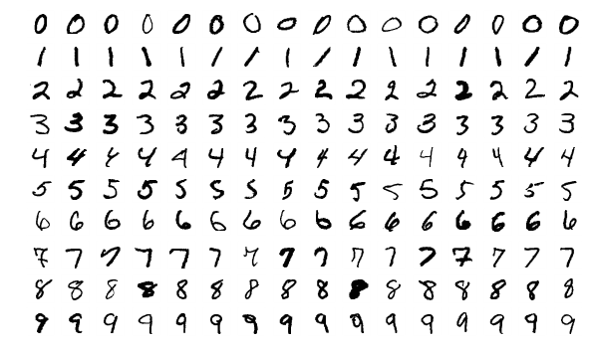
\includegraphics[height=2.5cm]{figs/mnist_examples.png}
                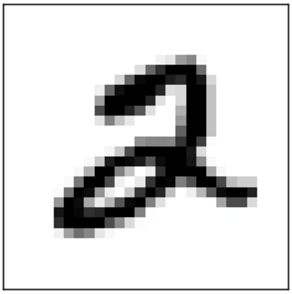
\includegraphics[height=2.5cm]{figs/mnist_example.png}    
            \end{center}
    \end{columns}
\end{frame}


\begin{frame}

    \frametitle{A Deeper Look at Experience}

    \begin{itemize}
        \item \textbf{Supervised Learning}: Question \& answer pairs.
        \item \textbf{Unsupervised Learning}: Looking for patterns.
        \item \textbf{Reinforcement Learning}: Interaction with environment.
    \end{itemize}

    % \begin{center}
    %     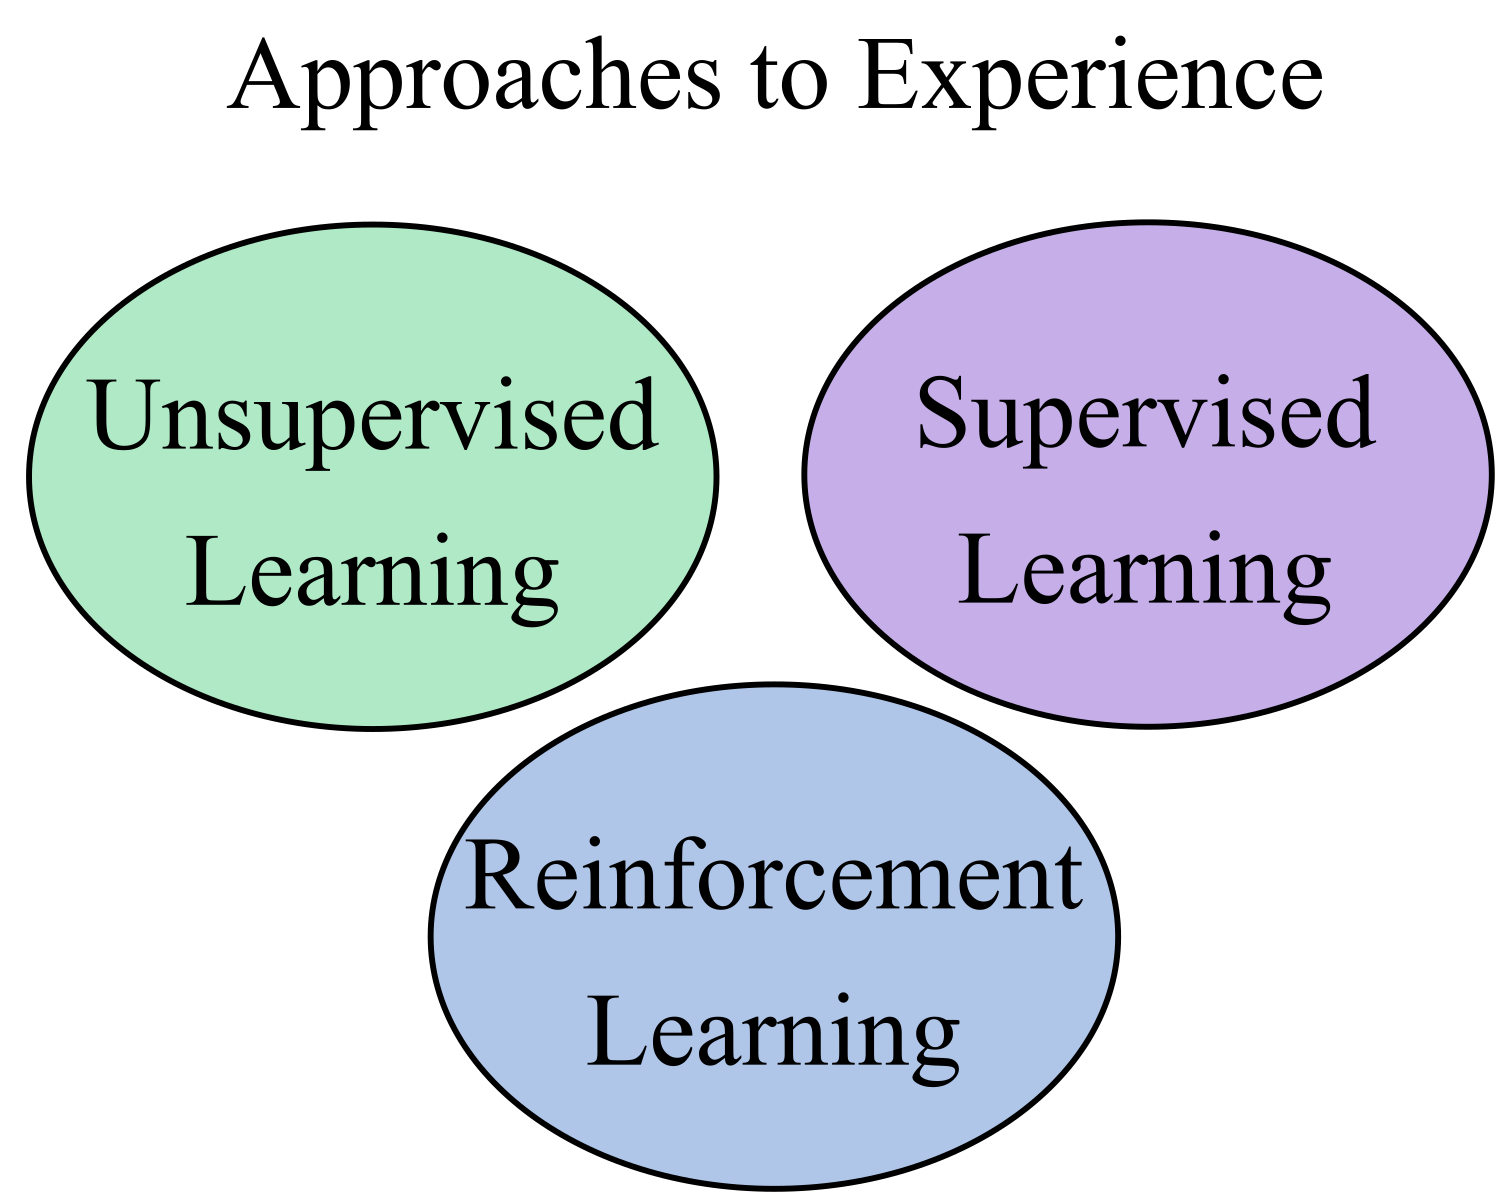
\includegraphics[height=5cm]{figs/experience.png}
    % \end{center}

\end{frame}


\begin{frame}

    \frametitle{General Approach to Supervised Deep Learning}

    \begin{enumerate}
        \item Acquire the data.
        \item Prepare the data.
        \item Split the data.
        \item Develop the Network Architecture.
        \item Select training hyperparamters.
        \item Train the network.
        \item Repeat steps 4 - 6 until satisfactory performance.
    \end{enumerate}

\end{frame}

\begin{frame}

    \frametitle{1. Acquire the Data}

    \begin{itemize}
        \item Can be a tedious and time consuming process.
        \item Generally not the case in engineering.
        \item Critical to understand the problem you are trying to solve.
    \end{itemize}

    \begin{center}
        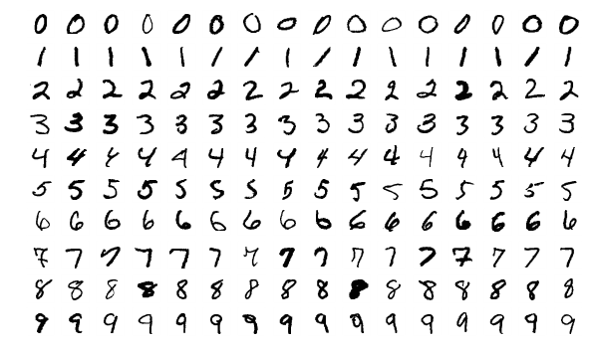
\includegraphics[height=4cm]{figs/mnist_examples.png}
    \end{center}

\end{frame}


\begin{frame}

    \frametitle{2. Prepare the Data}

    \begin{itemize}
        \item Clean the data
        \begin{itemize}
            \item get into some form of tensor.
            \item examples: one-hot encoding.
        \end{itemize}
        \item Normalize the data
        \begin{itemize}
            \item helps neural networks (NN) performance.
            \item store the normalization factors!
        \end{itemize}
        \item Feature Engineering
        \begin{itemize}
            \item help the network by extracting useful features.
        \end{itemize}
        \item Data Augmentation
        \begin{itemize}
            \item increase dataset size
            \item minimal computation effort
            \item but be careful.
        \end{itemize}
    \end{itemize}
\end{frame}

\begin{frame}
    \frametitle{3. Split the Data}

    \begin{itemize}
        \item Training Set
        \begin{itemize}
            \item typically 60 - 70\% of total data.
            \item used for model training.
        \end{itemize}
        \item Validation Set
        \begin{itemize}
            \item typically 10 - 20\% of total data.
            \item used during training for hyperparameter tuning.
            \item semi-objective measure of network performance.
            \item concern about information leakage.
        \end{itemize}
        \item Testing Set
        \begin{itemize}
            \item typically 20\% of total data.
            \item only used once at the very end.
            \item only objective measure of network performance.
        \end{itemize}

    \end{itemize}
\end{frame}

\begin{frame}
    \frametitle{4. Develop Network Architecture}

    \begin{itemize}
        \item Start with input and output shape.
        \item Remainder is up to the network designer.
        \item Remains an open question.
        \item Requires trial and error assessing performance using the validation set.
        \item examples: size, number, and types of hidden layers.
    \end{itemize}

    \vskip20pt

    Skip additional details for now …

\end{frame}

\begin{frame}
    \frametitle{5. Select Training Hyperparameters}

    \begin{itemize}
        \item Hyperparameters include:
        \begin{itemize}
            \item Optimization algorithm
            \begin{itemize}
                \item Examples: SGD, RMSProp, Adam.
            \end{itemize}
            \item Loss function
            \begin{itemize}
                \item Classification: Binary/Categorical Cross Entropy
                \item Regression: L1 Loss, L2 Loss
            \end{itemize}
            \item Batch size
            \begin{itemize}
                \item typically a factor of two.
                \item linked to the learning rate.
            \end{itemize}
            \item Learning Rate
            \begin{itemize}
                \item selected for good convergence for specific batch size
                \item helpful to use a learning rate schedule.
            \end{itemize}
            \item Number of Epochs
            \begin{itemize}
                \item number of cycles through training data.
                \item prevent over-fitting with early stopping
            \end{itemize}

        \end{itemize}

    \end{itemize}

    
\end{frame}

\begin{frame}
    \frametitle{6. Train}

    \begin{itemize}
        \item Training is a numerical optimization problem.
        \item The parameters of your network are updated to reduce your loss function.
        \item The analyst’s job is to monitor training.
        \item Primary concern is \textbf{overfitting}.
        \item \textbf{Underfitting} is also a concern and may indicate need for architecture changes.
    \end{itemize}

    \begin{center}
        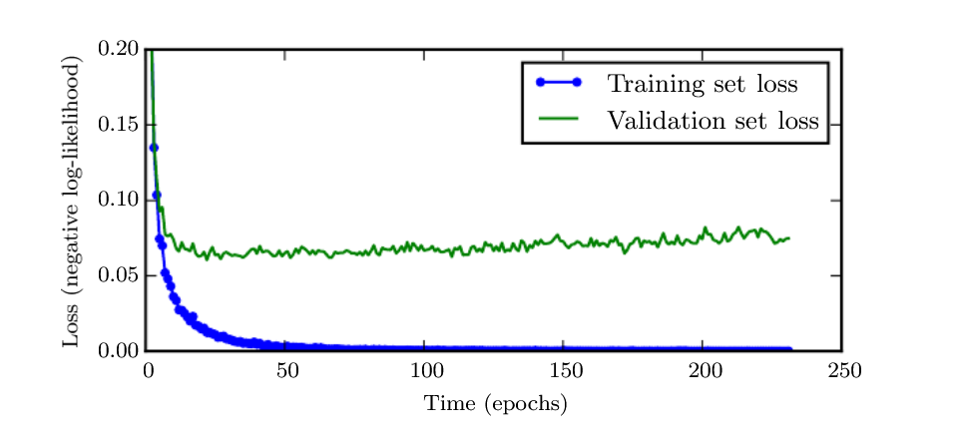
\includegraphics[height=4cm]{figs/train_val_example.png}
    \end{center}
    
\end{frame}

\begin{frame}[fragile]
    \frametitle{Practice Problem: MNIST}

    \begin{itemize}
        \item Use the Keras version of the MNIST dataset:
        \item Prepocess the data (do not worry about data augmentation for now).
        \item Try at least three different architectures.
        \item Try a variety (at least 10) hyperparameter combinations.
        \item Create plots of the learning curves for the different architecture and hyperparameters.
        \item Create a figure showing your predicted from 10 random samples from the testing set.
        \item Run test set only once you have decided on your best architecture and report accuracy.
    \end{itemize}
    \vskip20pt
    Some starter code:
    \begin{semiverbatim}
!pip install Keras
import keras          
data = keras.datasets.mnist.load_data()
(x_train, y_train), (x_test, y_test) = data
    \end{semiverbatim}    

\end{frame}

\end{document}